\documentclass{beamer}
\usetheme{metropolis} % Ou remplacez par votre thème préféré
\usepackage{amsmath, amsfonts, mathtools}
\usepackage{stmaryrd}
\usepackage{graphicx}
\usepackage{subcaption}
\usepackage{float}
\usepackage{tikz}
\usepackage{pgfplots}
\usepackage{bbold}
\usepackage{bm}  
\usepackage{bbm}
\usepackage{etoolbox}
\usepackage{array}
\usepackage{adjustbox}
\usepackage{caption}

\captionsetup{justification=centering}
\pgfplotsset{compat=1.18} % Version pour PGFPlots
\makeatletter
\patchcmd{\beamer@calculateheadfoot}{\insertcontinuationcount}{\relax}{}{}
\makeatother


\title{Multiway multiblock logistic regression to classify liver tumors from MRI images}
\author{SELVESTREL Alexandre}
\institute{
    Université Paris-Saclay, CNRS, CentraleSupélec, Laboratoire des signaux et systèmes\\[10 pt]
    \textbf{Supervisors :} Arthur Tenenhaus, Laurent Lebrusquet\\[10 pt]
    \textbf{Medical partner :} Henri Mondor hospital, radiologist: Sébastien Mulé
}
\date{\today}

\begin{document}

\begin{frame}
    \titlepage
\end{frame}

\begin{frame}
    \frametitle{Liver tumors classification}
    \begin{center}
        \textbf{$\mathbf{6}^{\text{th}}$ most widespread cancer and $\mathbf{4}^{\text{th}}$ mortality cause by cancer}\\
    \end{center}
    Classification:
    \begin{itemize}
        \item Hepatocellular Carcinoma (HCC): $75\%$ of cases, resection often possible\\[10 pt]
        \item CCK = Cholangiocarcinoma (CCK): $6\%$ of cases, resection difficult (possible $30\%$ of cases)\\[10 pt]
        \item Others: benign ($18 \%$ of cases) or Hepatoblastoma ($1 \%$ of cases)
    \end{itemize}
\end{frame}

\begin{frame}
    \frametitle{Difficulties for classification}
    \begin{itemize}
    \item No perfect method using RMI images (contrast, shape, size, location): disagreement between radiologists \\[15 pt]
    \item High alpha-fetoprotein indicate HCC, but not always.\\[15 pt]
    \item Biopsy: invasive and potentially lethal ($0.02 \%$ of patients)\\
    \end{itemize}
    \onslide<2->{
    \begin{center}
        But a lot of clues even without Biopsy $\rightarrow$ Machine Learning
    \end{center}
    Specifically: adapting existing methods to the structure of the data (tensors)
    }
\end{frame}

\begin{frame}
    \frametitle{Available data}

    $\bullet$ RMI images in 3D of liver tumors (arterial, portal, veinous -not used-, late)\\[5 pt]
    $\bullet$ gender\\[5 pt]
    $\bullet$ age at disease\\[30 pt]

    Same variables extracted from each RMI images... 3 times

    
\end{frame}


\begin{frame}
    \begin{figure}
        \centering
        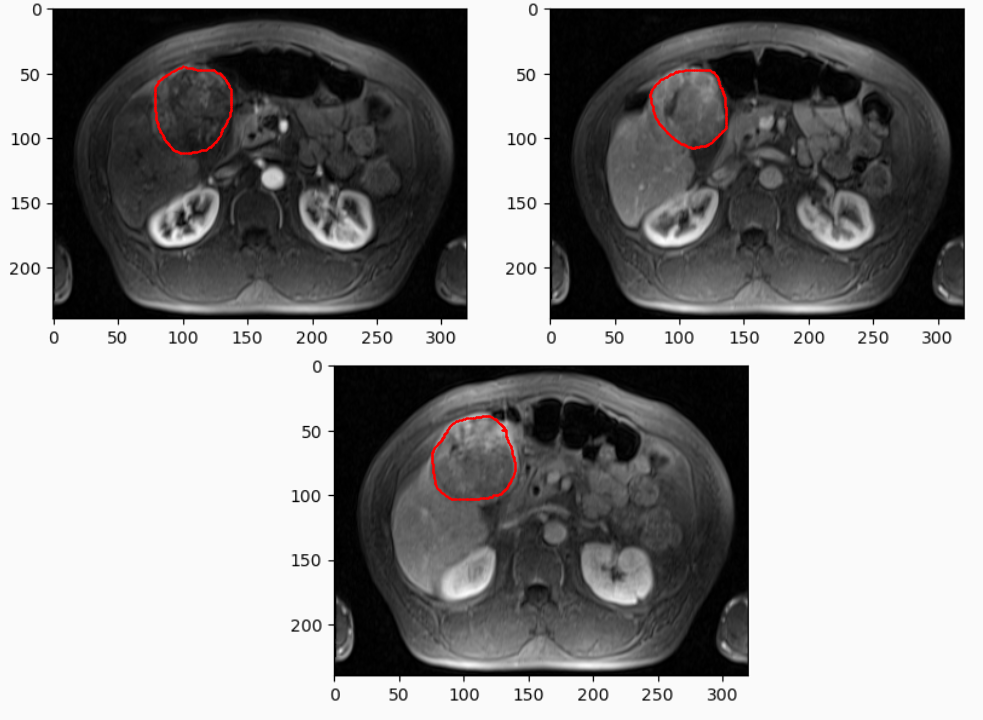
\includegraphics[scale = 0.215]{images/HCC.png}
        \caption{Example of RMI images of a HCC tumor (arterial, portal, late). More contrast in arterial}
    \end{figure}
\end{frame}

\begin{frame}
    \begin{figure}
        \centering
        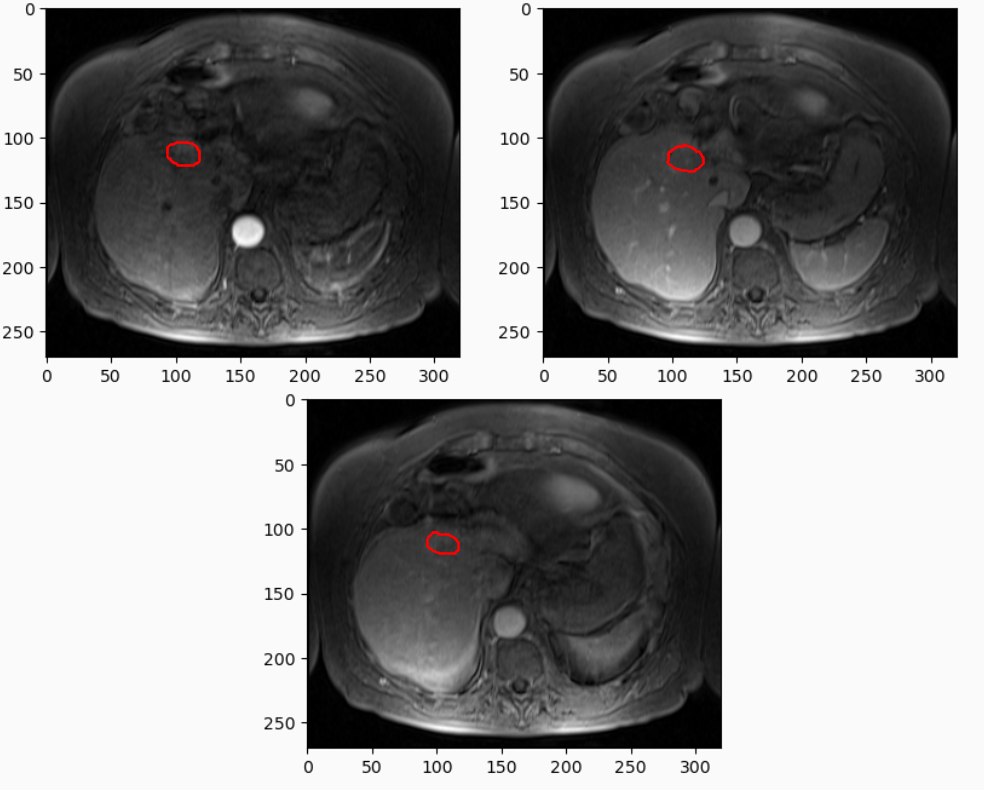
\includegraphics[scale = 0.215]{images/CCK.png}
        \caption{Example of RMI images of a CCK tumor (arterial, portal, late)}
    \end{figure}
\end{frame}


\begin{frame}
    \frametitle{Correlation matrix of the texture (GLDM) coefficients}
    Strong correlations between the imaging times for a given variable
    \begin{figure}
        \centering
        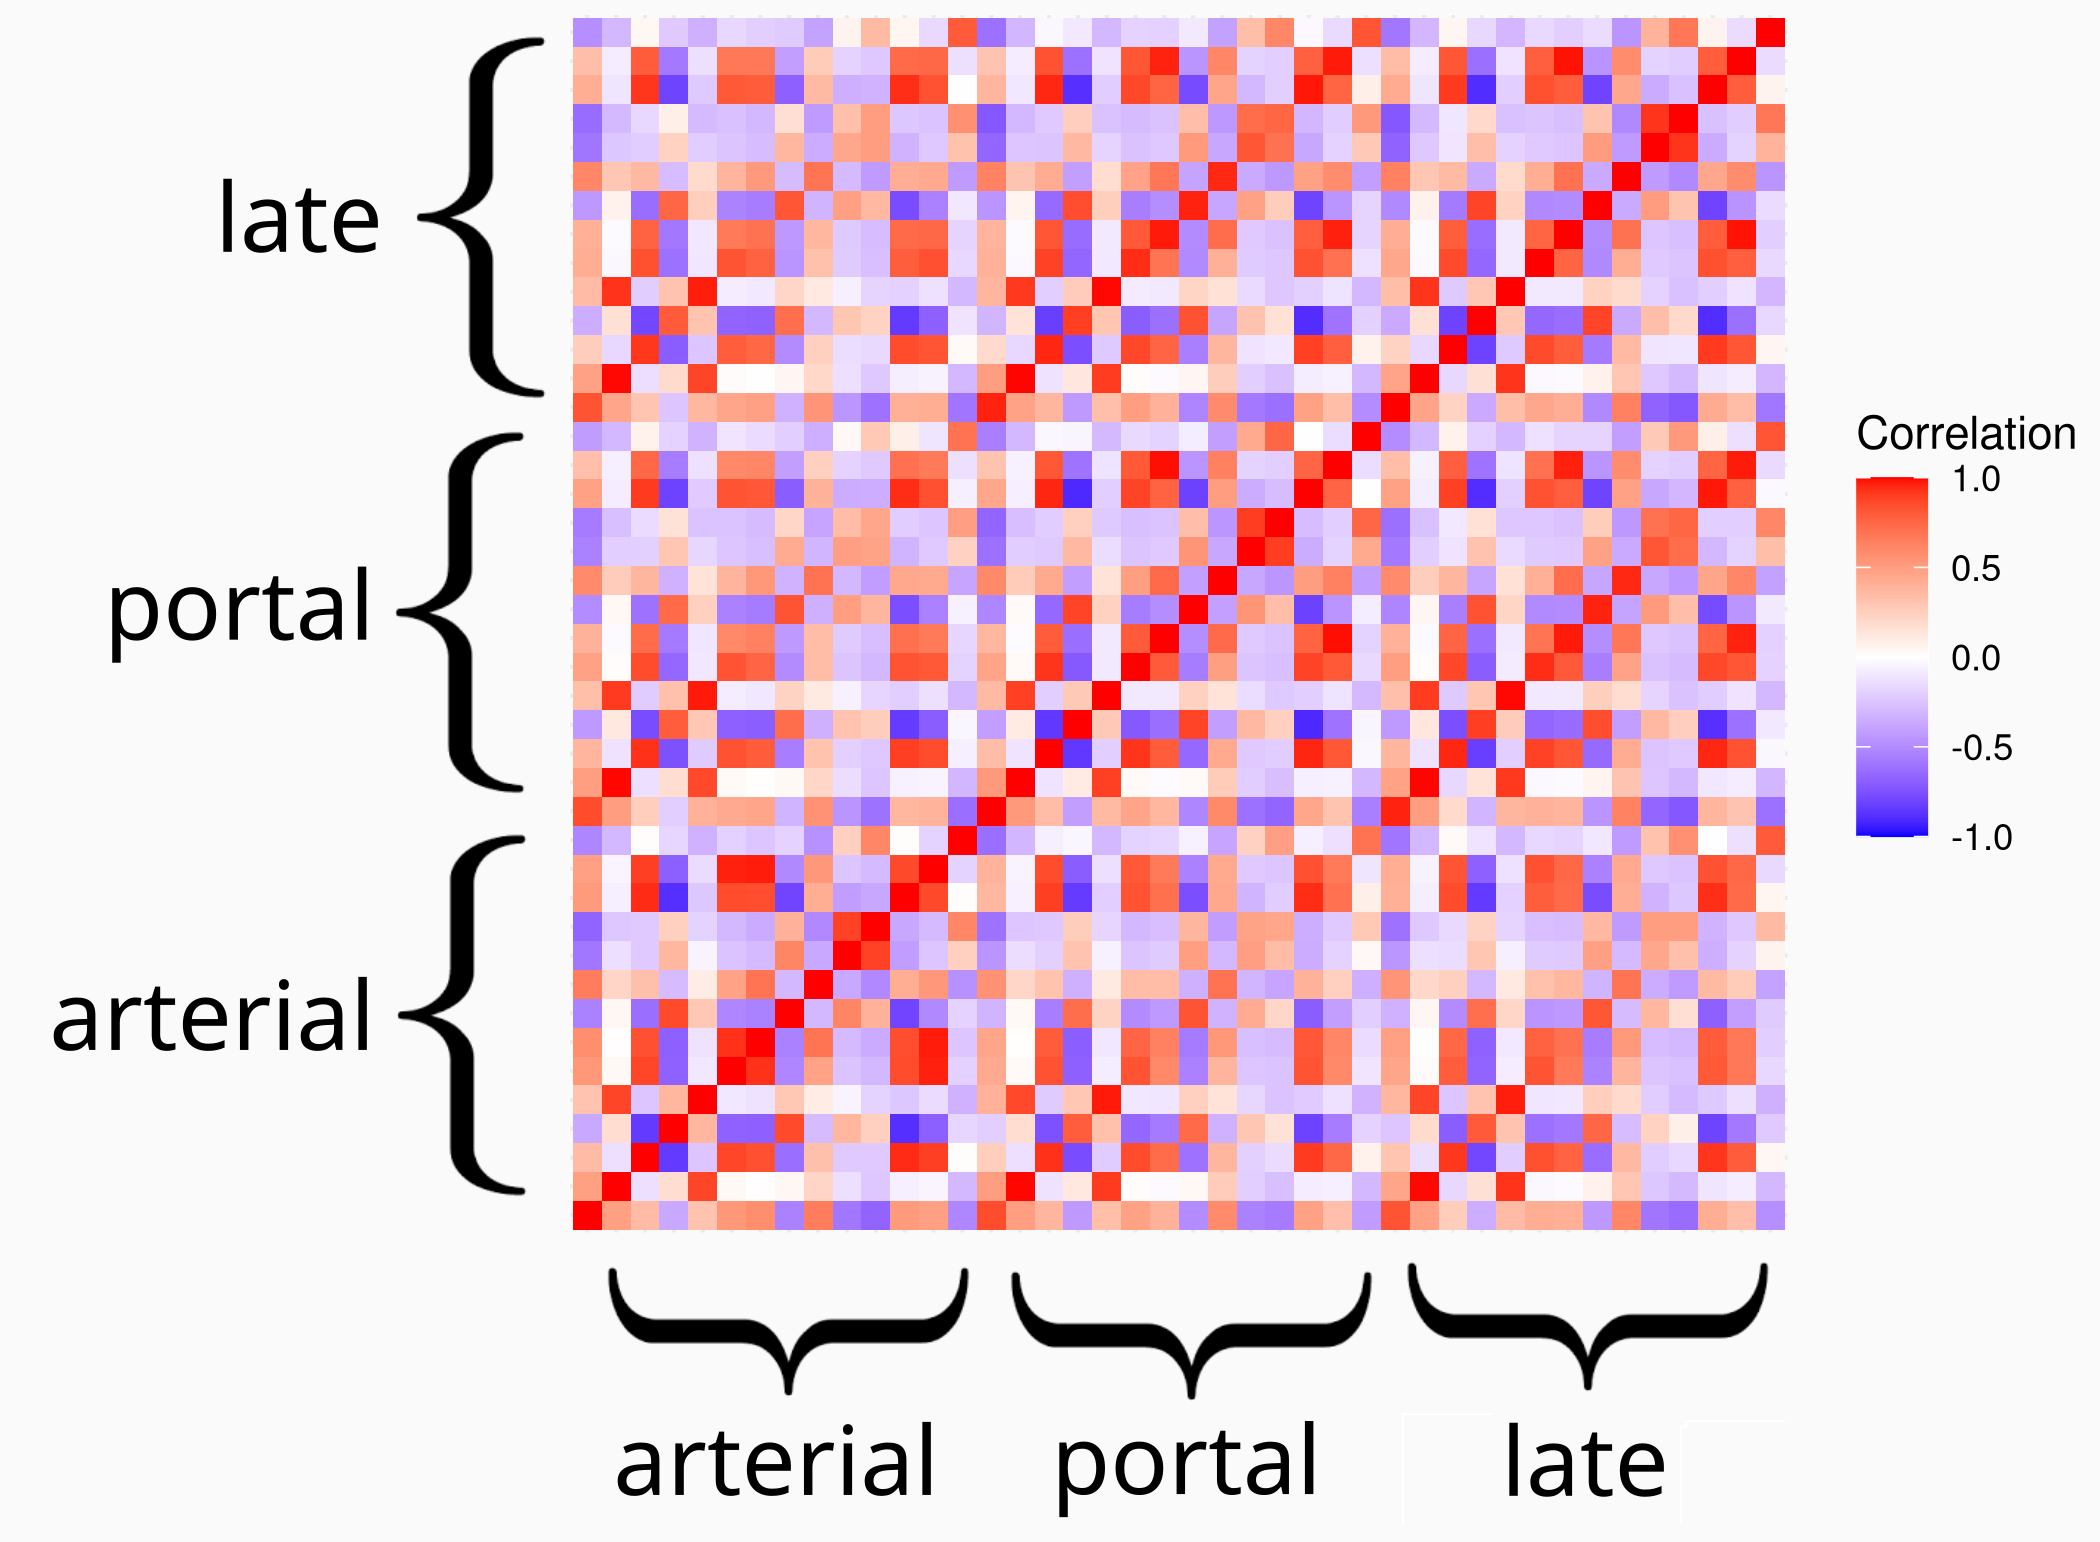
\includegraphics[scale = 0.1]{images/correlation.png}
        \caption{Correlation matrix of the texture coefficients elative to Gray Level Dependence Matrix (GLDM)}
    \end{figure}

\end{frame}

\begin{frame}
    \frametitle{Tensor data}
    Finding the best algorithm considering the structure of the data.
    \begin{figure}
        \centering
        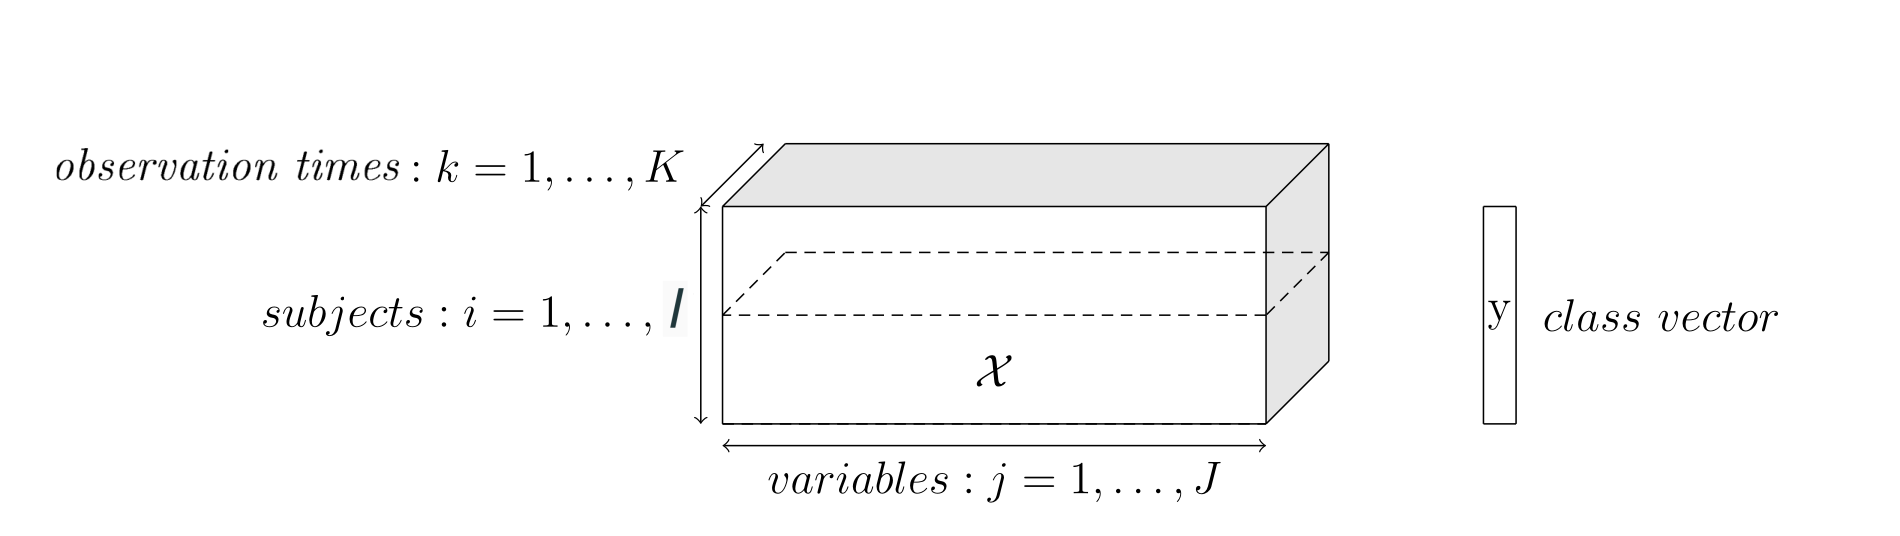
\includegraphics[scale = 0.3]{images/tensor.png}
        \caption{Type of data: tensorial}
    \end{figure}


\end{frame}

\begin{frame}
    \frametitle{Multibloc data}
    Features about pixel/voxel intensities, shape and texture: different natures
    \begin{figure}
        \centering
        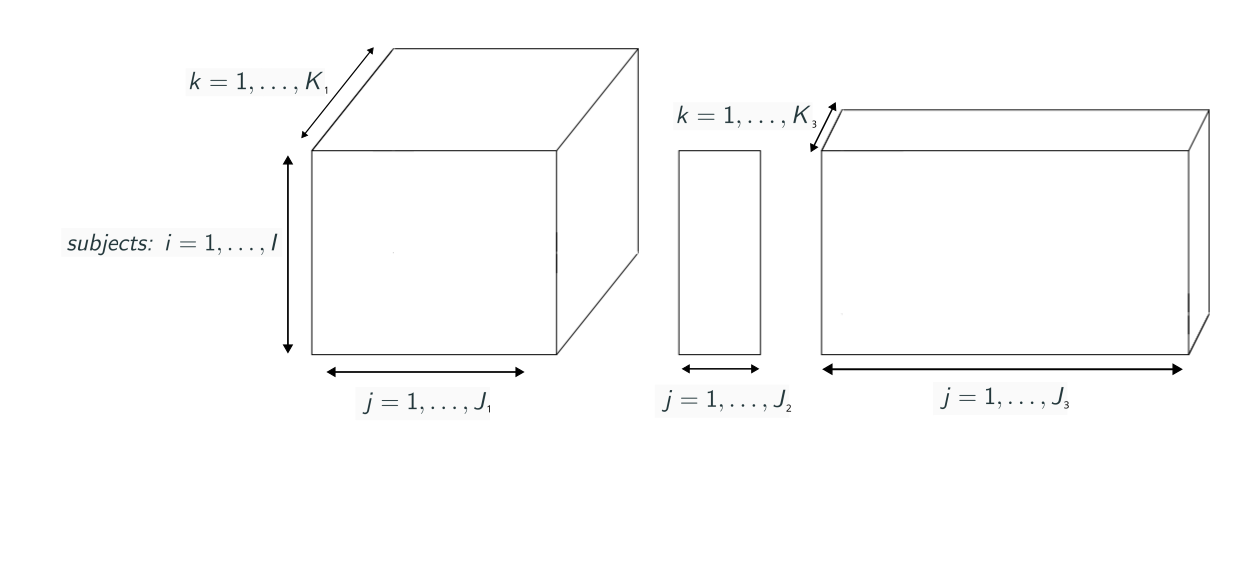
\includegraphics[scale = 0.35]{images/blocks.png}
        \caption{Type of data: multibloc}
    \end{figure}
\end{frame}



\begin{frame}
    \frametitle{Table of contents}
    \tableofcontents
\end{frame}

\begin{frame}
    \section{Machine learning models}
    \subsection{tabular models}
\end{frame}

\begin{frame}
    \frametitle{Logistic regression}
    $I$\\[10 pt]
    Classical machine learning (few data and explainable)\\[10 pt]

    $$P(Y = 1|x) = \frac{\exp(\beta_0 + \bm{x}^T\hspace{-2 pt}\bm{\beta})}{1 + \exp(\beta_0 + \bm{x}^T\hspace{-2 pt}\bm{\beta})}$$

    Defines a likelihood function $\mathcal{L}(\bm{\beta}) = \prod_{i = 1}^n P(Y_i = y_i|x_i)$\\[15 pt]

    function to minimize : $- \log(\mathcal{L}(\bm{\beta})) + \text{penalization}$ \\[15 pt]

    Penalization to avoid overfitting. In our case L1 norm (lasso)
\end{frame}

\begin{frame}
    \frametitle{Limitations of the logistic regression lasso}
        $\bullet$ Each feature impact considered independently (no link between the times). Adapting penalty would change nothing on this\\[15 pt]
        $\bullet$ Elimination of features without specific considerations for the same feature at other times/ other features at the same time\\[15 pt]

    \onslide<2->{

    
    2 main solutions:
    \begin{itemize}
        \item Preprocessing the data so it becomes tabular (equivalent to the approach chosen with latest data). But using only PCA + clustering: bad results
        \item Adapting the model to the structure of the data (aim of the internship)
    \end{itemize}
    }

\end{frame}

\subsection{tensormodels}
\begin{frame}
    \frametitle{Tensor regression models}
    Idea: each variable and mode has its own influence on the prediction (i.e. on $\bm{\beta}$) \cite{multi_rank_1}.\\[10 pt]

    For $J$ variables observed following $M$ modes (time, depth ...)
    $$\beta_{j,k_1,\hdots,k_M} = \beta_j^J\beta_{k_1}^{K_1} \hdots \beta_{k_m}^{K_M}$$
    \onslide<2->{
    reformulation with $\bm{\beta}$ as a vector:
    \begin{align*}
        \bm{\beta} &= [\beta_{1,1,\hdots,1}, \beta_{2,1,\hdots,1} \, \hdots \, \beta_{1,2,\hdots,1} \, \hdots \, \beta_{J,K_1,\hdots,K_M} ]^T \hspace{5 pt} (\text{lexicographic order})\\[5 pt]
        &= \bm{\beta}^{K_M} \otimes \hdots \otimes \bm{\beta}^{K_1} \otimes  \bm{\beta}^{J} \hspace{5 pt} (\text{Kronecker product}) 
    \end{align*}
Concatenate non tensor coefficients at the end of the Kronecker structure}
\end{frame}

\begin{frame}
    \frametitle{Limits of rank $1$}
    $\bm{\beta}^{K_M} \otimes \hdots \otimes \bm{\beta}^{K_1} \otimes  \bm{\beta}^{J}$  is only rank $1$\\[10 pt]
    In 2D :
    \begin{figure}
        \centering
        \begin{minipage}{0.3\textwidth}
            \centering
            
\includegraphics[width=\textwidth]{images/square.png}
            \caption{\centering Example of rank 1 pictogram (only 0 and 1)}
        \end{minipage}
        \hspace{0.1\textwidth}
        \begin{minipage}{0.4\textwidth}
            \centering
            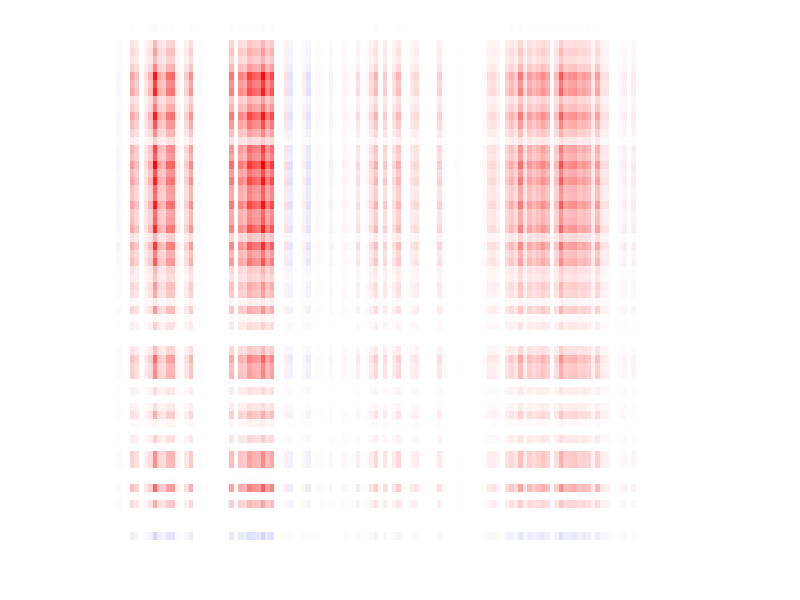
\includegraphics[width=\textwidth]{images/picto_500/heatmap_logistic_multibloc_simu_500_multiway.png}
            \caption{\centering Example of rank 1 matrix (all values allowed)}
        \end{minipage}
    \end{figure}

\end{frame}

\begin{frame}
    \frametitle{Rank R multiway logistic regression}
    Allowing any rank $R$ \cite{multi_rank_r}
    $$\bm{\beta} = \sum\limits_{r = 1}^R \bm{\beta}_r^{K_M} \otimes \hdots \otimes \bm{\beta}_r^{K_1} \otimes  \bm{\beta}_r^{J}$$

    Chosen penalization: $\sum\limits_{r = 1}^R \lVert \bm{\beta}_r^{K_M} \otimes \hdots \otimes \bm{\beta}_r^{K_1} \otimes  \bm{\beta}_r^{J} \rVert_1$
    \begin{itemize}
        \item L1-type penlization: encourage sparsity of each $\bm{\beta}_r^{K_m}$ and $\bm{\beta}_r^J$\\[10 pt]
        \item Allows efficient optimization, considering the $\bm{\beta}$-structure
    \end{itemize}
\end{frame}

\begin{frame}
 \frametitle{grouping by blocs}

 \textbf{Problem}: Several groups of variables of different natures (first order, shape, texture). But $\bm{\beta}_r^{K_1} \, \hdots, \bm{\beta}_r^J$ common to all groups. \\[15 pt]

 \textbf{Solution} : Separating each group of variables in different blocks (tensors), with own $\bm{\beta}_r^{K_1} \, \hdots, \bm{\beta}_r^J$ for each block.

 \begin{figure}
        \centering
        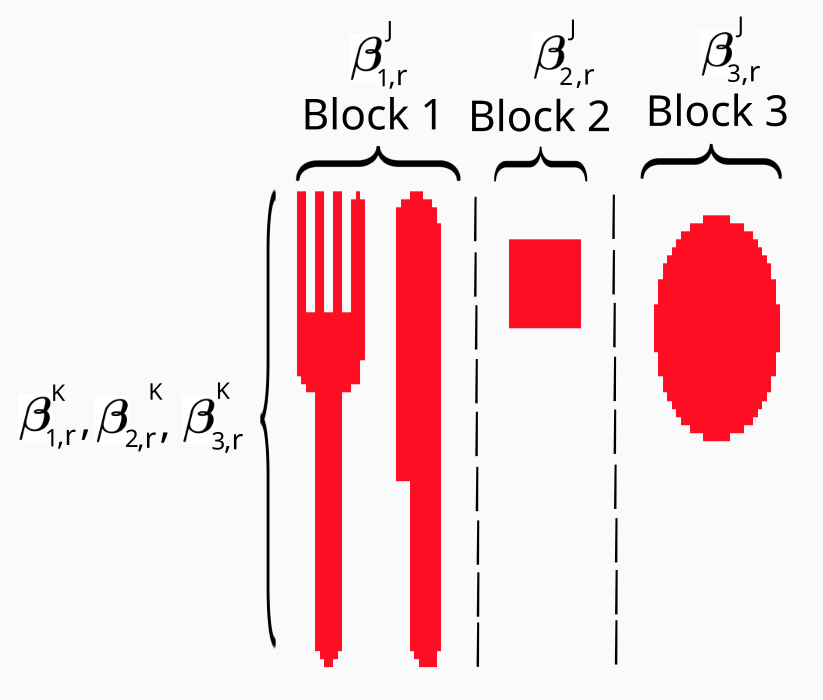
\includegraphics[scale = 0.165]{images/picto_explic.png}
        \caption{Separation by blocks of a pictogram}
  \end{figure}

\end{frame}

\begin{frame}
    \frametitle{Multiway Multiblock Logistic Regression (MMLR)}

    For L blocks, when $\bm{\beta}$  of order $2$ (extension rank $R$ straightforward):

    $$    \bm{\beta} = \left[ \sum\limits_{r = 1}^{R_1} \bm{\beta}_{(1,r)}^{K} \otimes \bm{\beta}_{(1,r)}^J;   \; \; \hdots  \; \; ;\, \sum\limits_{r = 1}^{R_L}\bm{\beta}_{(L,r)}^K \otimes \bm{\beta}_{(L,r)}^J \right] $$
    \phantom{a}\\
    Allows having different orders for $2$ different blocks,  e.g.: averaging over time only 1 block\\[10 pt]
    Same penalization as multiway model but summed by block
\end{frame}

\begin{frame}
    \section{Simulations}    
\end{frame}

\begin{frame}
    \frametitle{Parameters to control:}
    \begin{itemize}
        \item Difficulty of the classification (overlap between classes, distance between means of classes etc ...)\\[12 pt]
        \item Balance between classes\\[12 pt]
        \item Structure of the regression coefficients $\bm{\beta}$ (several blocks)\\[12 pt] 
        \item Quality of the classification (AUC)\\[12 pt]
        \item Quality of the reconstruction of $\bm{\beta}$ (pictograms)
    \end{itemize}
\end{frame}

\begin{frame}
    \frametitle{Data generation}
    Chose the $\bm{\beta}$ to be reconstructed (pictograms)\\[10 pt]
    Generate the $(\mathbf{x}_i)_{i \in \llbracket 1, I\rrbracket}$ with 2 multivariate normal laws of means $\bm{\mu}_1$ and $\bm{\mu}_2$ and common covariance matrix $\bm{\Sigma}$ such that:
    \begin{itemize}
        \item $\bm{\mu}_2 - \bm{\mu}_1$ colinear to $\bm{\beta}$\\[10 pt]
        \item One of the principal axis of $\bm{\Sigma}$ colinear to $\bm{\beta}$
    \end{itemize}
    Separation of classes linked with eigenvalues of $\bm{\Sigma}$ (to be compared with $\lVert\bm{\mu}_2 - \bm{\mu}_1 \rVert$)
\end{frame}

\begin{frame}
    \frametitle{Example in 2D}

    \begin{figure}
        \centering
        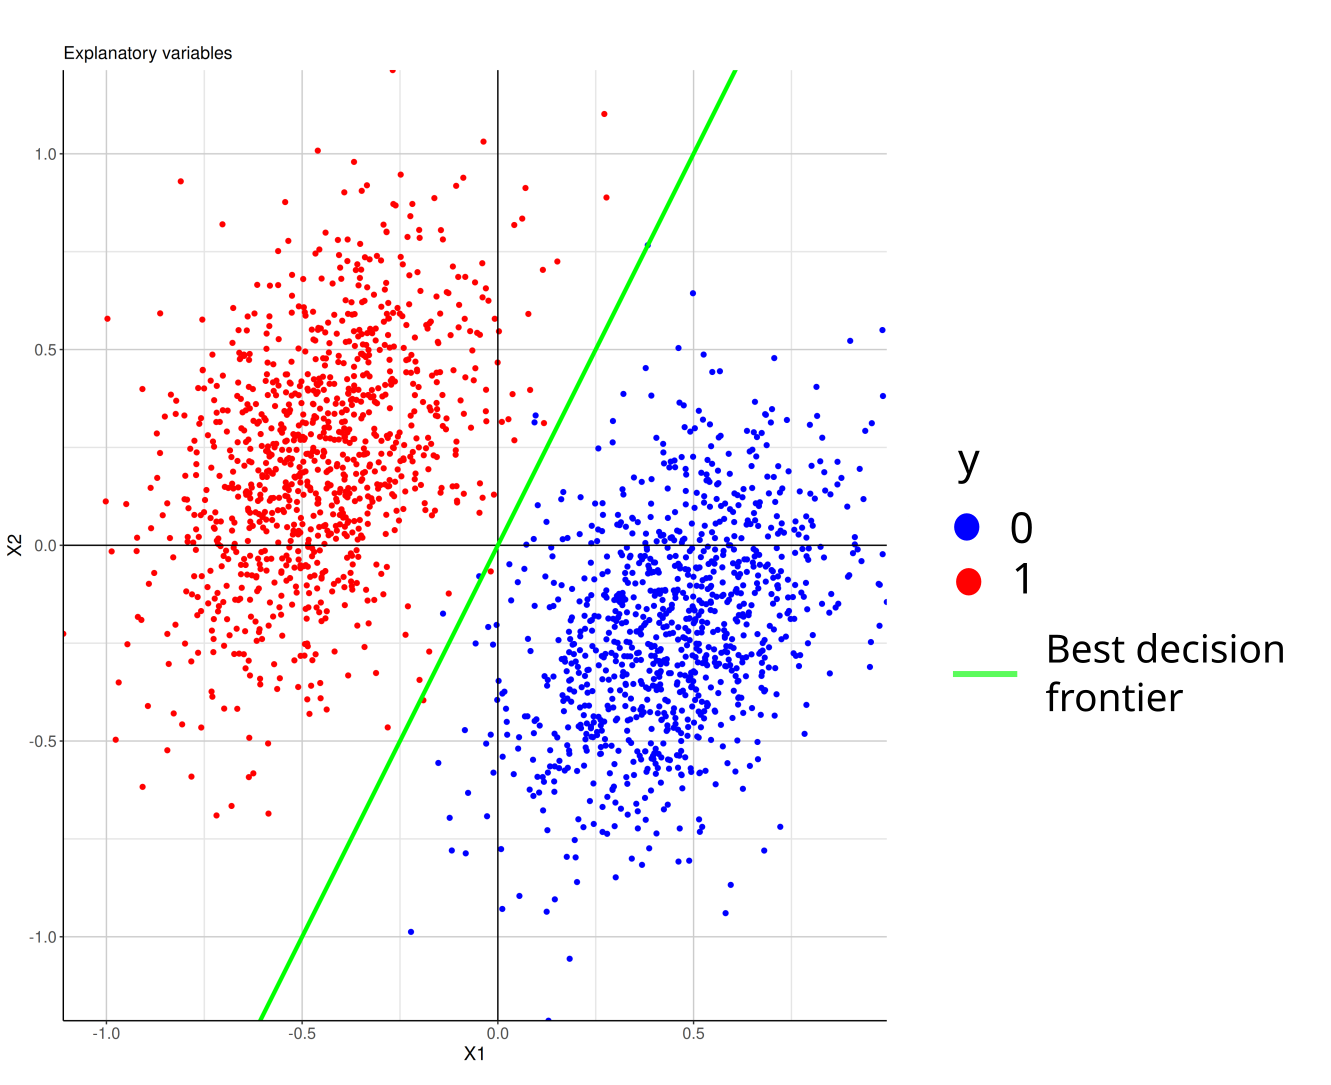
\includegraphics[scale = 0.16]{images/2D.png}
        \caption{Example of explanatory variables for $\bm{\beta} = (-2,1)$}
    \end{figure}
\end{frame}

\begin{frame}
    \frametitle{AUC simulated data}
    \begin{figure}
        \begin{table}[H]
            \centering
            \caption{AUC for each model on simulated data for 3000 individuals}
            \label{tab:result_simul}
            \renewcommand{\arraystretch}{1.2} 
            \begin{adjustbox}{center}
            \begin{tabular}{|>{\centering\arraybackslash}m{1.4cm}|>{\centering\arraybackslash}m{1.1cm}|>{\centering\arraybackslash}m{1.1cm}|>{\centering\arraybackslash}m{1.1cm}|>{\centering\arraybackslash}m{1.1cm}|>{\centering\arraybackslash}m{1.1cm}|>{\centering\arraybackslash}m{1.1cm}|}
                \cline{1-7}
                $(\sigma_{\bm{\beta}}$, $\sigma_{\text{noise}})$ & lasso & g. l (blocs) & g.l (mode)& g.l (var) & tensor & tensor blocks\\
                \cline{1-7} 
                (0.1,0.5) & 0.83 & 0.86 & 0.94 & 0.94 & 0.99 & 0.99 \\
                \cline{1-7}
                (0.1,0.8) & 0.63 & 0.64 & 0.68 & 0.68 & 0.93 & 0.99 \\
                \cline{1-7}
            \end{tabular}
        \end{adjustbox}
        \end{table}
    \end{figure}
\end{frame}

\begin{frame}
    \frametitle{Reconstructed $\bm{\beta}$}
    \begin{figure}[H]
        \centering
        \begin{minipage}{0.35\textwidth}
            \centering
            \subfloat[lasso $(\sigma_{\bm{\beta}}, \sigma_{\text{noise}}) = (0.1,0.5) $\label{fig:3000simple}]{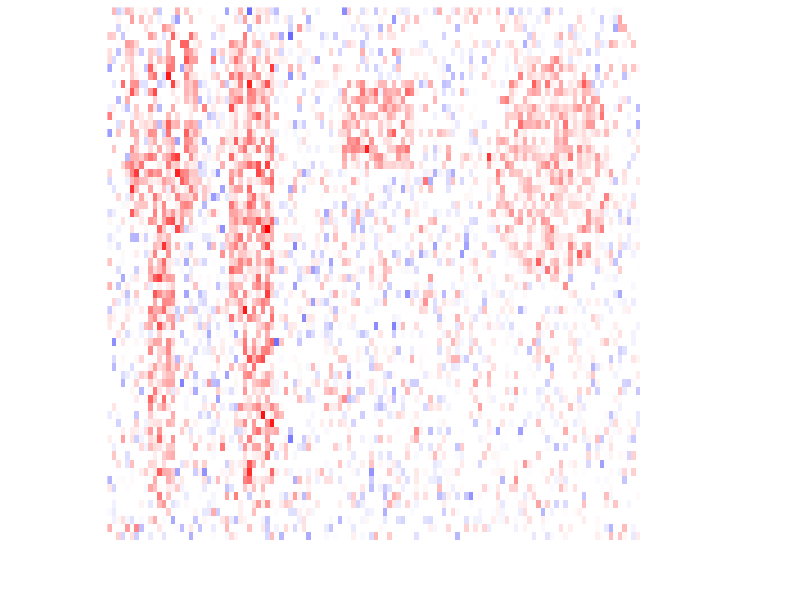
\includegraphics[width=\textwidth]{images/heatmap_logistique_simple_simu_4000.png}}
        \end{minipage}
        \hspace{0.05\textwidth} % Ajuster l'espace entre les images
        \begin{minipage}{0.35\textwidth}
            \centering
            \subfloat[multiway multiblock $(\sigma_{\bm{\beta}}, \sigma_{\text{noise}}) = (0.1,0.5) $\label{fig:multiblock}]{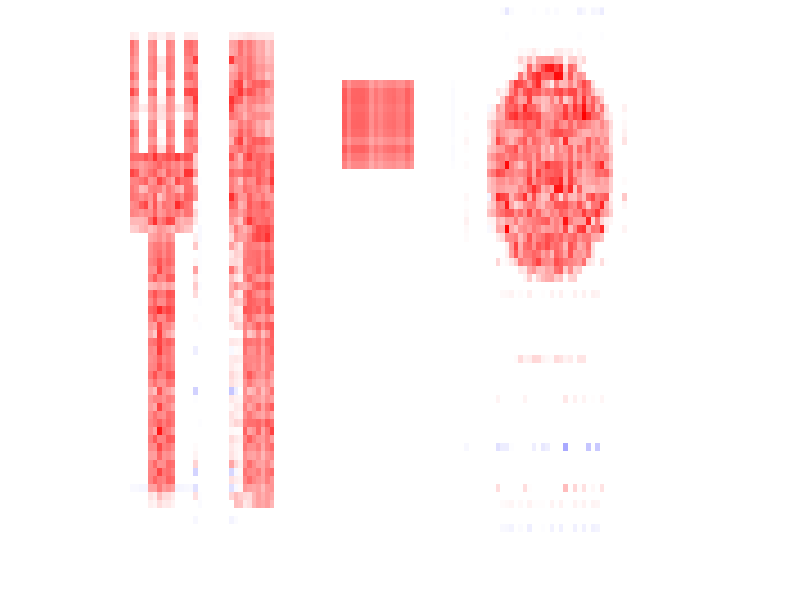
\includegraphics[width=\textwidth]{images/heatmap_logistic_multibloc_simu_4000.png}}
        \end{minipage}
        \begin{minipage}{0.33\textwidth}
            \centering
            \subfloat[multiway $(\sigma_{\bm{\beta}}, \sigma_{\text{noise}}) = (0.1,0.8) $\label{fig:easy_multiway}]{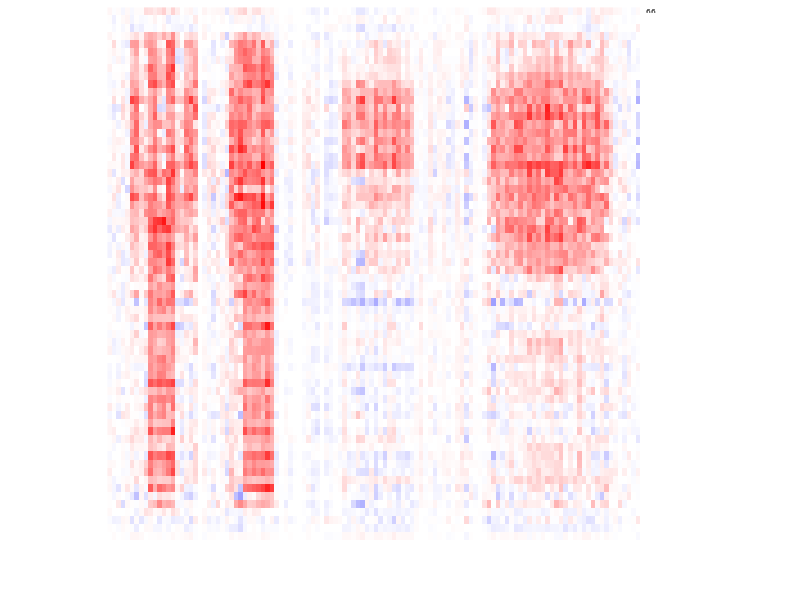
\includegraphics[width=\textwidth]{images/heatmap_logistic_multibloc_simu_4000_medium_easy_multiway.png}}
        \end{minipage}
        \hspace{10 pt}
        \begin{minipage}{0.33\textwidth}
            \centering
            \subfloat[multiway multiblock $(\sigma_{\bm{\beta}}, \sigma_{\text{noise}}) = (0.1,0.8) $\label{fig:easy_multiblock}]{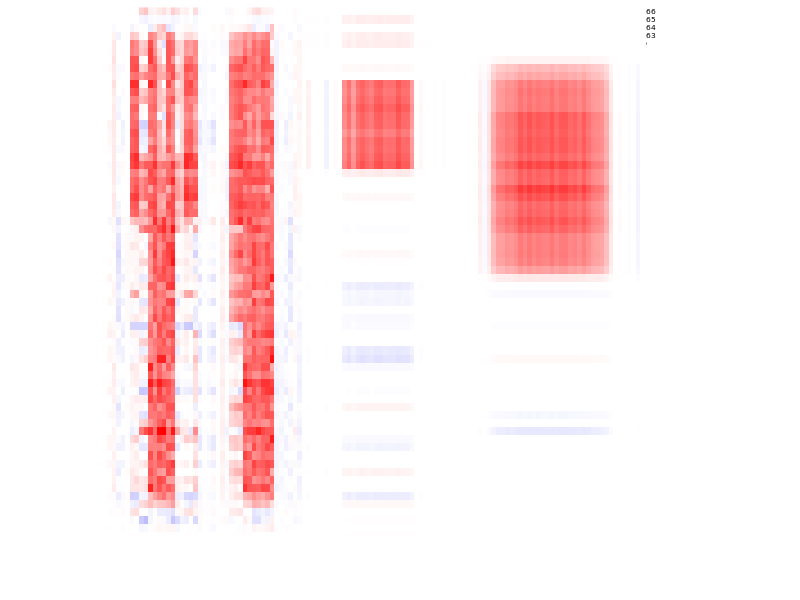
\includegraphics[width=\textwidth]{images/heatmap_logistic_multibloc_simu_4000_medium_easy.png}}
        \end{minipage}
    \end{figure}
\end{frame}

\begin{frame}
    \section{real data}
    \subsection{with pyradiomics}
\end{frame}

\begin{frame}
    \frametitle{Features extraction with pyradiomics}
    Extraction of $\simeq  100$ features (about intensities, shape, texture) for each $2$D or $3$D image.\\[10 pt]
    Difficulties: Which spacing? Which slices if 2D?\\[25 pt]
    \onslide<2->{\textbf{In 3D}:
    \begin{itemize}
        \item Common spacing\\[5 pt]
        \item Average shape over time
    \end{itemize}
    }
\end{frame}

\begin{frame}
    \frametitle{Features extraction in 2D}
    \vspace{5 pt}
    Slices along z axis $\rightarrow$ same spacing along $(x,y)$\\[5 pt]
    \textbf{But:} No common spacing along $z$  
    \begin{figure}
        \centering
        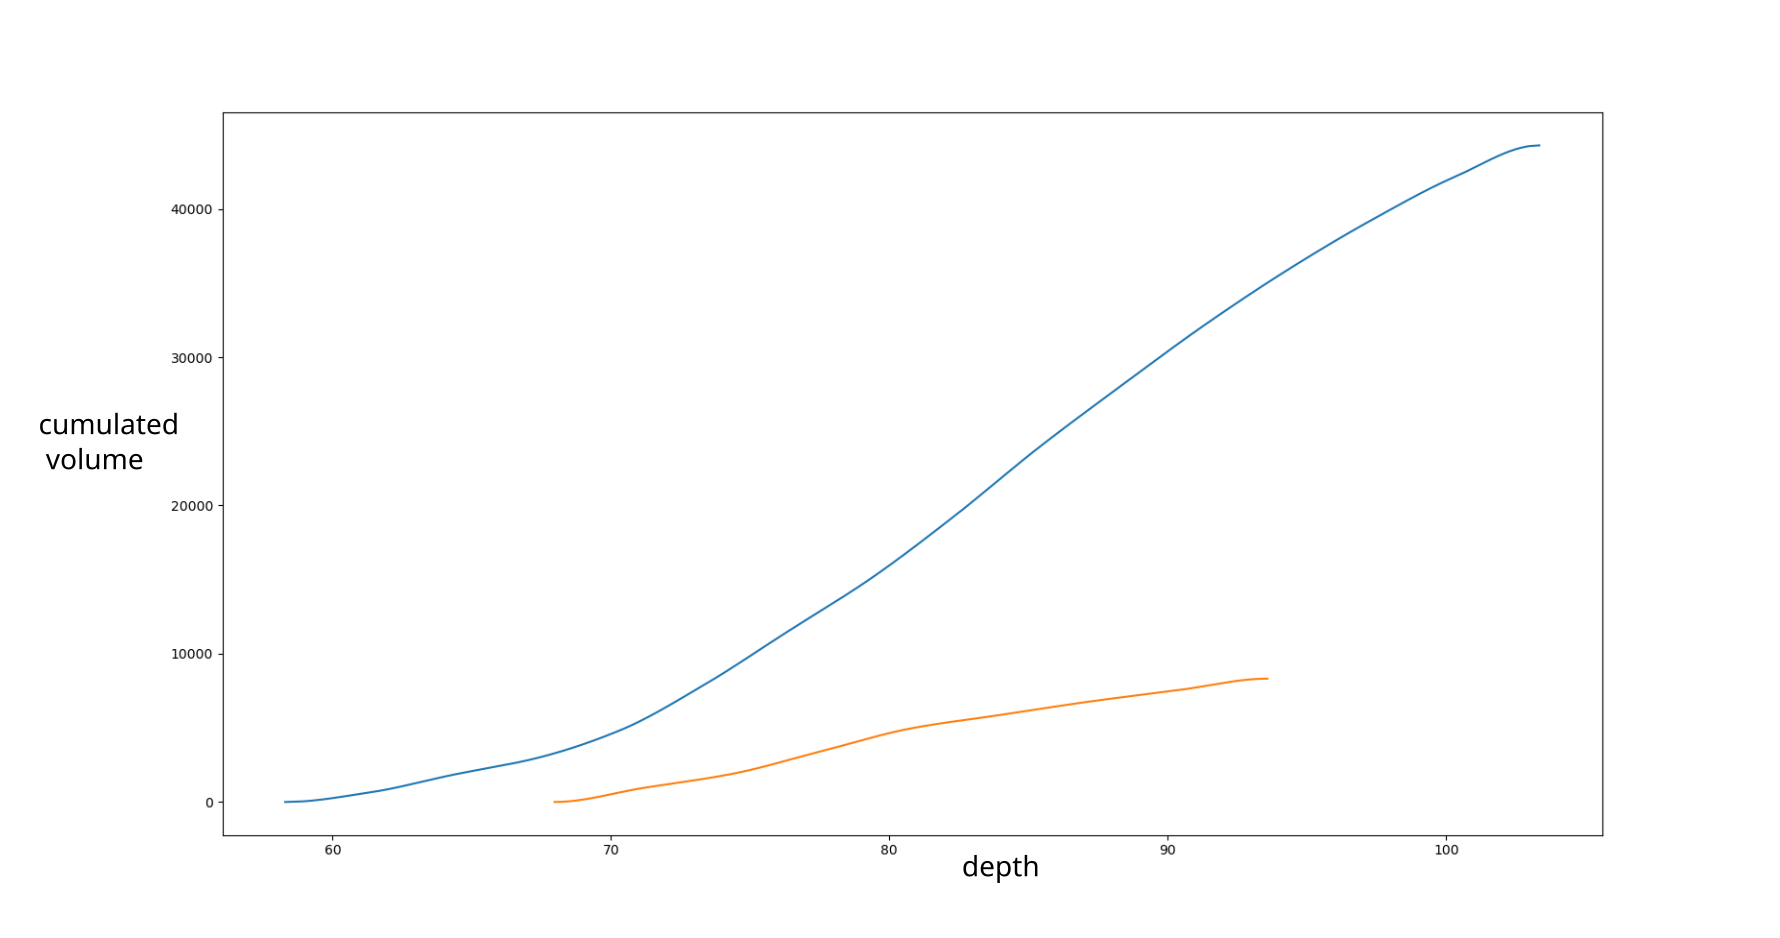
\includegraphics[scale = 0.18]{images/curves_area.png}
        \caption{Curves of the cumulated volume of tumor (in $mm^3$) as a function of the depth travelled in the liver (in $mm$) for 2 tumors during arterial phase}
    \end{figure}
\end{frame}

\begin{frame}
    \frametitle{Features extraction in 2D}
    Solution: Selecting $5$ slices equally spaced along the cumulated volume axis
    \begin{figure}
        \centering
        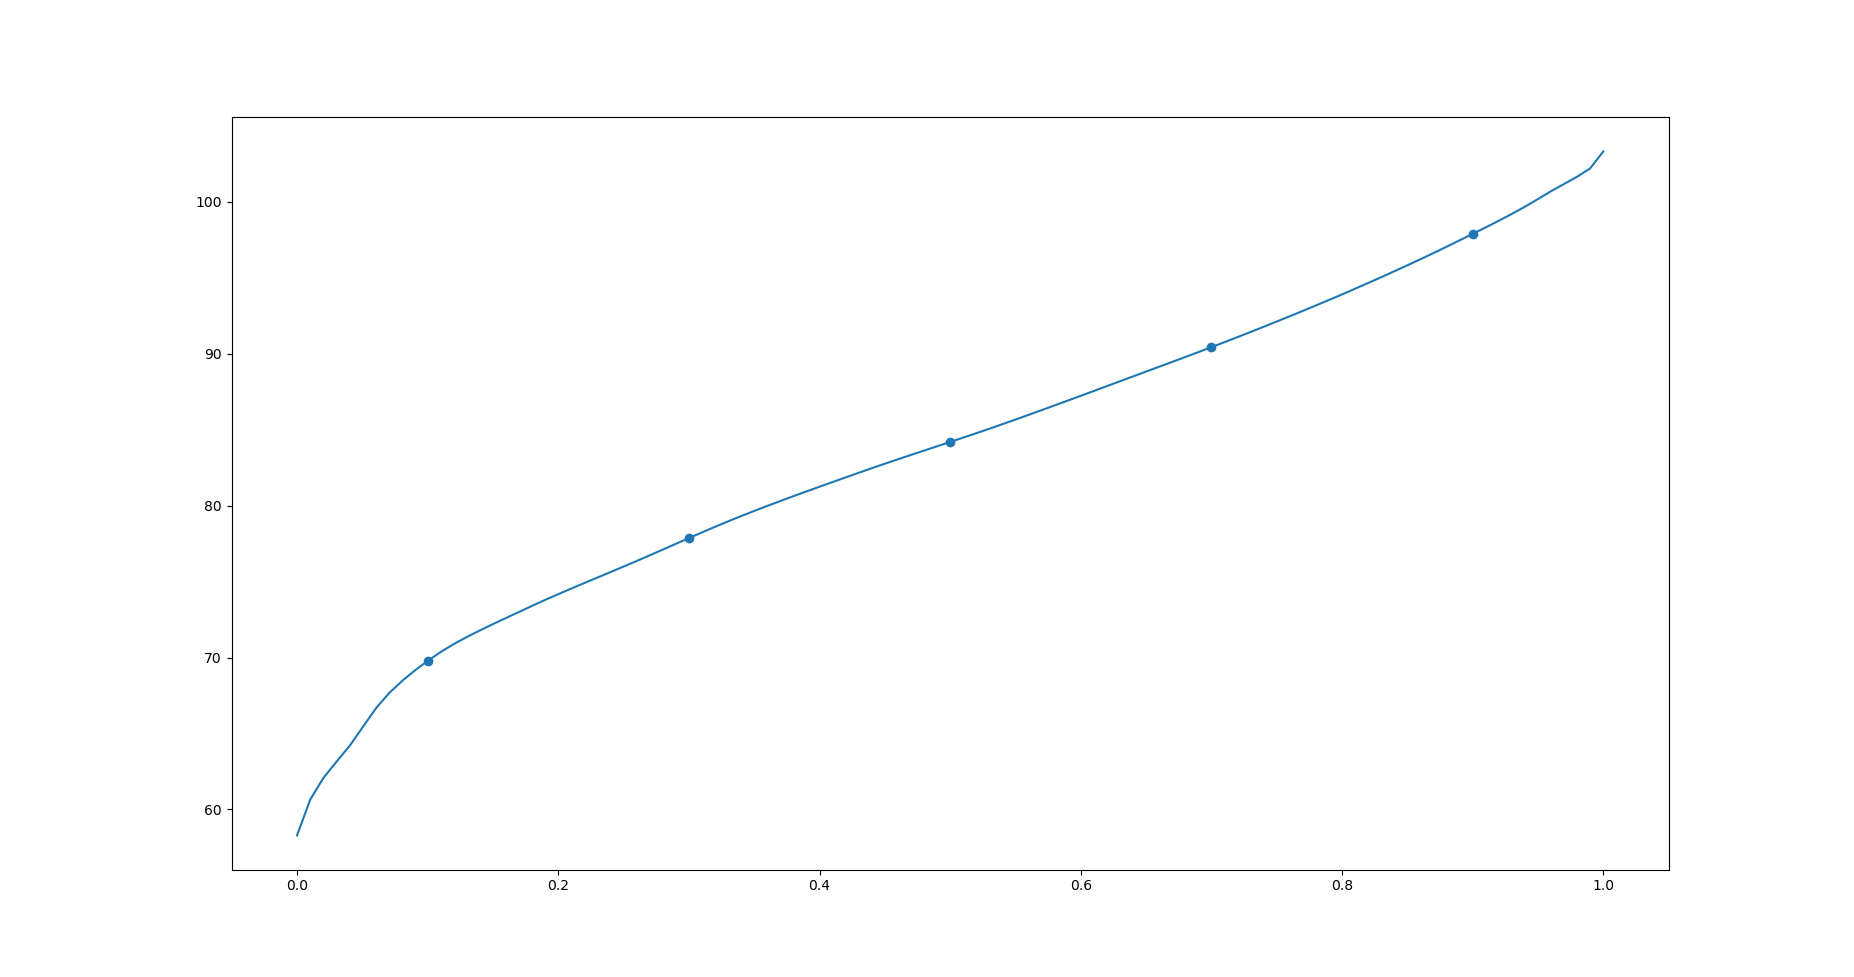
\includegraphics[scale = 0.15]{images/curve_points.png}
        \caption{Curve of the depth travelled in the liver  (in $mm$) as a function of the standardized cumulated volume of the tumor. The points represent the selected slices.}
    \end{figure}
\end{frame}

\begin{frame}
    \frametitle{Results}
    \begin{table}[H]
        \centering
        \label{tab:result_real}
        \renewcommand{\arraystretch}{1.2} 
        \begin{adjustbox}{center}
        \begin{tabular}{|>{\centering\arraybackslash}m{1.4cm}|>{\centering\arraybackslash}m{1.1cm}|>{\centering\arraybackslash}m{1.1cm}|>{\centering\arraybackslash}m{1.1cm}|>{\centering\arraybackslash}m{1.1cm}|>{\centering\arraybackslash}m{1.1cm}|>{\centering\arraybackslash}m{1.1cm}|}
            \cline{1-7}
            Type of data & lasso & g.l. (block) & g.l. (time)& g.l. (var) & tensor & tensor blocks\\
            \cline{1-7} 
            3D & $0.74 \pm 0.04$& $0.78 \pm 0.03$ & $0.76 \pm 0.03$ & $0.73 \pm 0.03$ & $0.77 \pm 0.03$ & $0.77 \pm 0.03$ \\
            \cline{1-7}
    
        \end{tabular}
        
    \end{adjustbox}
    \parbox{0.9\textwidth}{
    \vspace{0.2 cm}    
    \centering \small Area under curve (AUC) on 3D real data}
    \vspace{0.3 cm}
    
    \begin{adjustbox}{center}
    \begin{tabular}{|>{\centering\arraybackslash}m{1.2cm}|>{\centering\arraybackslash}m{1cm}|>{\centering\arraybackslash}m{1cm}|>{\centering\arraybackslash}m{1cm}|>{\centering\arraybackslash}m{1cm}|>{\centering\arraybackslash}m{1cm}|>{\centering\arraybackslash}m{1cm}|>{\centering\arraybackslash}m{1cm}|}
        \cline{1-8}
        Type of data & lasso & g.l. (block) & g.l. (slice)& g.l. (time)& g.l. (var) & tensor & tensor blocks\\
        \cline{1-8} 
        2D & $0.73 \pm 0.03$ & $0.71 \pm 0.03$ & $0.70 \pm 0.04$ & $0.71 \pm 0.03 $  & $0.71 \pm 0.03$ & $0.66 \pm 0.04$ & $0.71 \pm 0.03$ \\
        \cline{1-8}
    \end{tabular}
    \end{adjustbox}
    \parbox{0.9\textwidth}{
    \vspace{0.2 cm}    
    \centering \small Area under curve (AUC) on 2D real data}
    \end{table}
\end{frame}

\subsection{latest data}

\begin{frame}
    \frametitle{Latest data}
    13 binary features determined by radiologists (late enhancement, non peripheral washout etc...) + sex\\[10 pt]
    With lasso model:
    \begin{itemize}
        \item AUC: $0.97 \pm 0.02$\\[10 pt]
        \item balanced accurcy: $0.88 \pm 0.05$
        \end{itemize}
    Would be interesting to test other models...
\end{frame}

\begin{frame}
    \frametitle{features importance}
    \begin{figure}
        \centering
        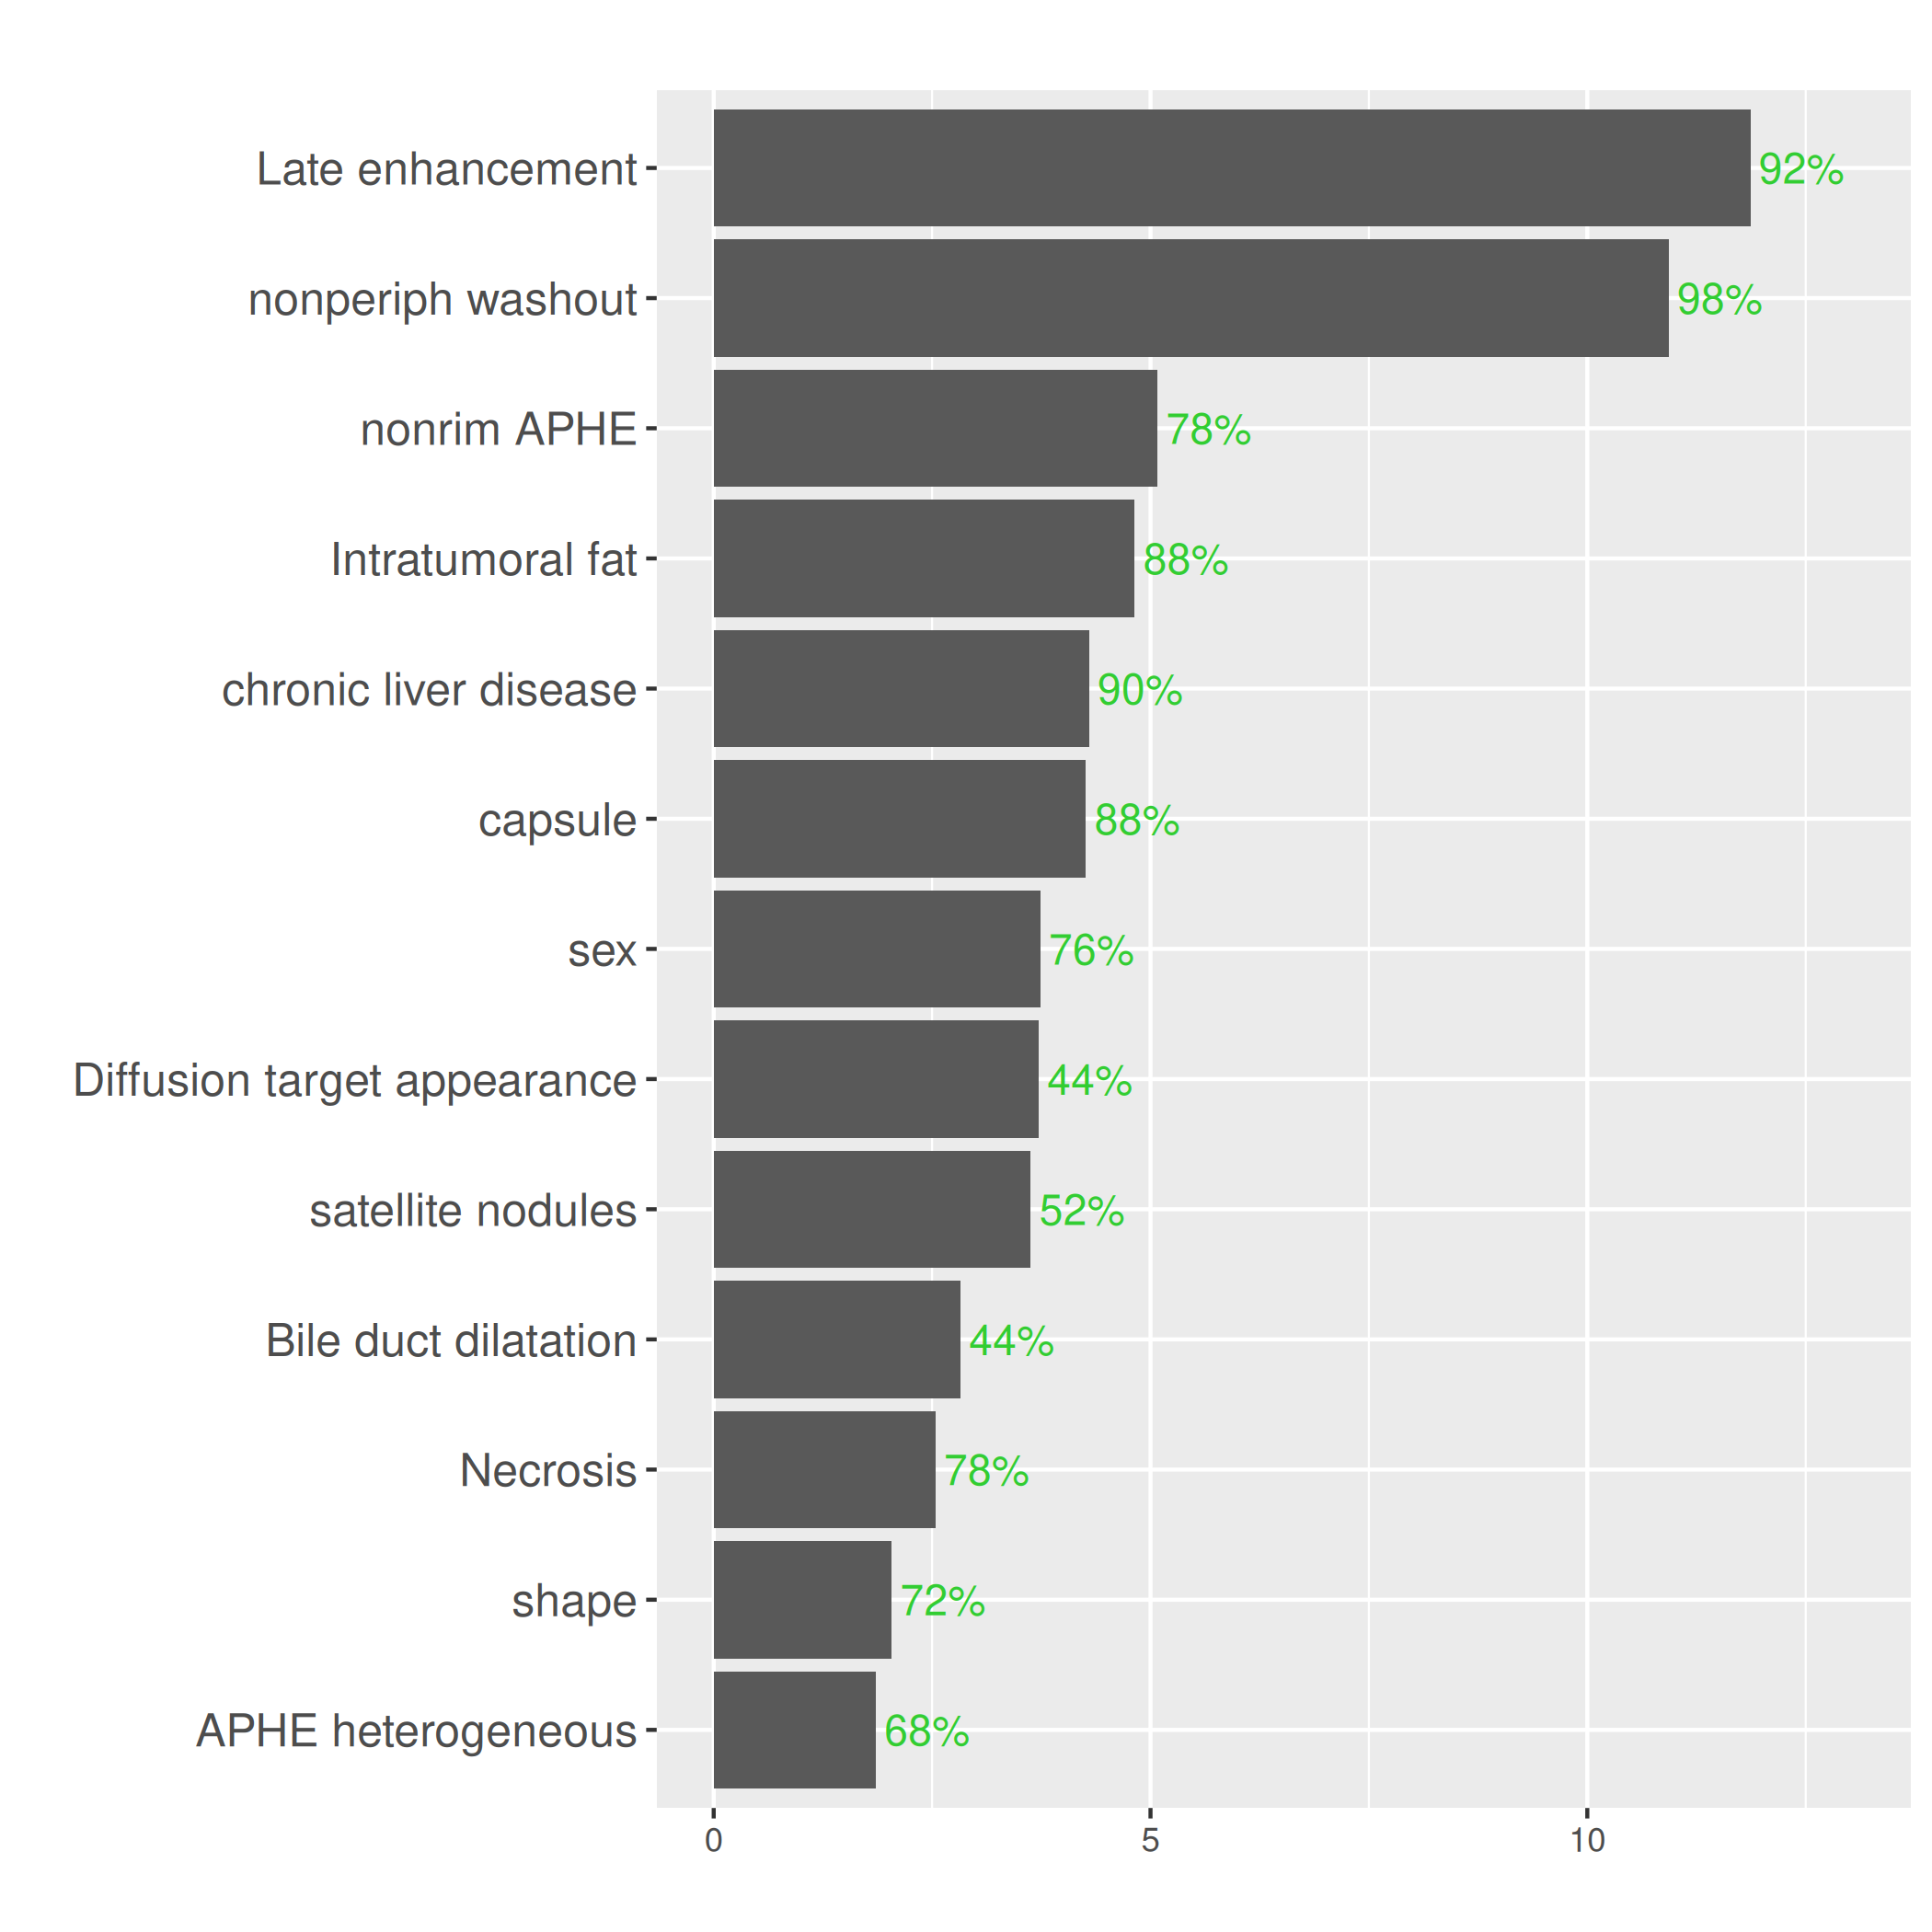
\includegraphics[scale = 0.38]{images/barplot_final.png}
        \caption{Features importance with lasso (in green percentage of runs with non null coefficient)}
    \end{figure}
\end{frame}

\begin{frame}
    \frametitle{Possible extensions}
    Testing other penalizations (group lasso, elastic net)\\[10 pt]
    Extending the multiblock approach to other classical machine learning algorithms (other GLMs, SVM etc...)\\[10 pt]
    Testing other models on the latest data (in order to obtain a model that can be deployed in the hospital)\\[10 pt]
    Implementing the multiblock code in C forincreased speed (currently quite slowin R)
\end{frame}

\begin{frame}
    \section{Retrospective Analysis}
\end{frame}

\begin{frame}
    \frametitle{Impact of the internship on me}
    Direct impact: continuing in thesis (increase in motivation for research activities)\\[10 pt]
    Soft skills in machine learning: become more critical vs results, searching for other data whenever possible\\[10 pt]
    Being part of a team in a scientific context (not only 1 supervisor): importance of communication and reporting (even when no writen documents)\\[10 pt]
    The reasearch in machine learning: an accessible world
\end{frame}


\begin{frame}
    \frametitle{Consequences of the internship}
    A promising framework for the diagnosis of liver tumors\\[10 pt]
    The simulation part of an article on the multiblock multiway logistic regression\\[10 pt]
    More information about the correct context for using that kind of models\\[10 pt]
    An ethically positive impact (controllable deployment, a precise need, no replacement of humans...)
    
\end{frame}

\begin{frame}
    \frametitle{Conclusion}
    A good representation of a research work (and its challenges)\\[10 pt]
    Supportive, available and Calm supervision (evn as deadlines approach)\\[10 pt]
    Looking forward to continuing in this direction
\end{frame}

\begin{frame}
\section*{bibliography}
\end{frame}


\begin{frame}[allowframebreaks] 
    \bibliographystyle{plain}
    \bibliography{bibliography.bib} 
    \end{frame}



\end{document}